\section{Results}
\label{sec:results}
The results from the experiments in the project report [??],
showed that the query expansion implementation had about 2 times longer latency compared to the baseline implementation.
The latency were measured from the request left the user to the response from the server arrived.

All the results show that the first request is often the slowest.
After the initial request the respons is cached by Lucene and makes all the subsequent requests a lot faster.

\subsection{Lucene Results}
About 50\% increased latency with the Lucene implementation.
Can see that Lucene heavily caches search result.
The first initial results often is a lot slower than the subsequent searces.

\subsection{Elasticsearch Experiment Results}
To evaluate the performance of the plugin developed a few tests were conducted.
All of the tests were done in two different ways,
one prewaring the cache and one without prewaring the cache.


\begin{figure}[h!]
  \centering 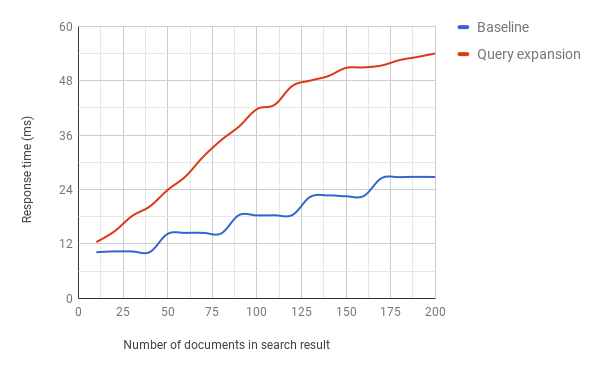
\includegraphics[width=1\linewidth]{img/result-vary-result-size.png}
  \caption{Overview of the different measurements used when evaluating the implementation.}
  \label{fig:result-vary-result-size}
\end{figure}

\begin{figure}[h!]
  \centering 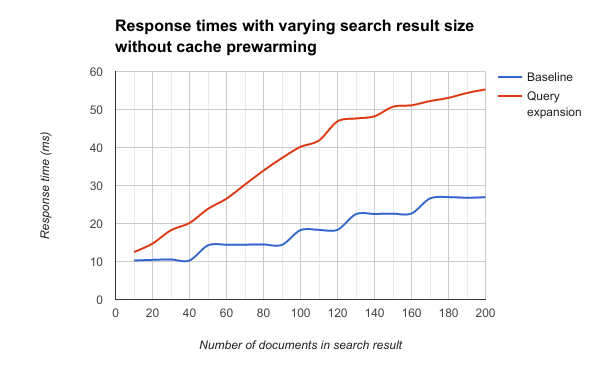
\includegraphics[width=1\linewidth]{img/result-vary-result-size-without-cache.png}
  \caption{Overview of the different measurements used when evaluating the implementation.}
  \label{fig:result-vary-result-size}
\end{figure}
